\documentclass[pdflatex,referee,lineno,sn-basic]{sn-jnl}

\usepackage{graphicx}%
\usepackage{multirow}%
\usepackage{amsmath,amssymb,amsfonts}%
\usepackage{amsthm}%
\usepackage{mathrsfs}%
\usepackage[title]{appendix}%
\usepackage{xcolor}%
\usepackage{textcomp}%
\usepackage{manyfoot}%
\usepackage{booktabs}%
\usepackage{array}%
\usepackage{tabularx}%
% floats are never set above the text that introduces them
\usepackage{flafter}%
% figures and tables are set in the text flow, right after the paragraph that introduces them
\makeatletter\providecommand\captionof[1]{\def\@captype{#1}\caption}\makeatother

\graphicspath{{figures/}}
\raggedbottom

% breakurl works only with pdflatex; other engines set reference URLs with \url
\usepackage{iftex}
\ifPDFTeX\else\AtBeginDocument{\let\burl\url}\fi
\hypersetup{pdftitle={Drift Detection, Diagnosis and Reliability Analysis for Deployed Machine Learning Models}, pdfauthor={Rahul Guhagarkar, Nathan Cherian, Alok Pal, Akul Patre, Sanjay Mirchandani}}

\begin{document}

\title[Drift Detection, Diagnosis and Reliability Analysis for Deployed Machine Learning Models]{Drift Detection, Diagnosis and Reliability Analysis for Deployed Machine Learning Models}

\author*[1]{\fnm{Rahul} \sur{Guhagarkar}}\email{2023.rahul.guhagarkar@ves.ac.in}
\author[1]{\fnm{Nathan} \sur{Cherian}}
\author[1]{\fnm{Alok} \sur{Pal}}
\author[1]{\fnm{Akul} \sur{Patre}}
\author[1]{\fnm{Sanjay} \sur{Mirchandani}}

\affil*[1]{\orgdiv{Department of Computer Engineering}, \orgname{Vivekanand Education Society's Institute of Technology}, \orgaddress{\street{Hashu Advani Memorial Complex, Collector's Colony, Chembur}, \city{Mumbai}, \postcode{400074}, \country{India}}}

\abstract{\textbf{Background:} Deployed machine learning models lose accuracy when production data drift away from the training data. Monitoring tools raise an alarm when this happens but seldom say what kind of drift occurred, although the right response depends on it: covariate shift calls for reweighting, prior shift for recalibration, concept drift for fresh labels and label noise for a check of the labeling process. This paper presents Data Drift Autopsy, an end-to-end monitoring pipeline that detects drift, estimates the lost accuracy without labels, locates the shifted features, names the drift type, scores the trust due to each prediction and advises whether a cheap retrain will help. At its heart sits a diagnosis made only of hypothesis tests, all held to one family-wise error rate. Its first stage uses no labels and tells covariate shift from prior shift. The second stage is new: given a few hundred late labels, it asks whether the errors have moved in a way the model's own confidence cannot account for, the mark that sets concept drift apart from label noise.\par \textbf{Results:} With drift injected into two census tasks and two model families, the diagnosis named the type in 85.7 to 94.3\% of windows, ahead of common monitoring rules. A learned meta-classifier did better on drift it had seen, yet fell to 31.1 to 51.2\% on held-out drift mechanisms, where our tests still reached 62.4 to 81.5\%. On four real datasets with documented changes, the pipeline flagged no control window and pointed to the known events.\par \textbf{Conclusions:} Hypothesis tests with a stated error rate can name the drift type, which decides the right response, from label-free tests and a few hundred late labels. Unlike a learned meta-classifier, the procedure carries over to held-out drift, because the tests encode the definitions of the types.}

\keywords{concept drift, label shift, model monitoring, drift diagnosis, hypothesis testing}

\maketitle


\section{Background}\label{sec:intro}

Nobody announces it when a deployed classifier starts to slip. The production data simply wander away from the training data, while the labels that would expose the loss tend to turn up weeks or months later~\citep{rabanser2019failing}. A monitor has to catch the change and make sense of it before those labels exist.

Existing monitors do the first part of that job well. They flag a changed distribution~\citep{rabanser2019failing} and give a fair estimate of how much accuracy has gone~\citep{garg2022atc,kivimaki2025performance}. Far fewer say what kind of change took place. That gap matters, since each kind has its own remedy. Moreno-Torres et al.~\citeyearpar{moreno2012unifying} distinguish three types of dataset shift. Under covariate shift the inputs drift but the mapping from inputs to labels holds, so reweighting the training data is often enough. Under prior shift it is only the class balance that moves, which recalibration usually fixes. Concept drift alters the mapping itself; nothing short of fresh labels will repair it. To these we add label noise as a fourth type. Here the labels used to grade the model are themselves corrupted, so the fault lies in how labels are collected rather than in the model.

Telling these types apart is harder than detecting that something changed. Covariate shift and prior shift both move the inputs and the predictions. Concept drift and label noise, on the other hand, leave the inputs as they were, so no test that looks only at unlabeled data can see them.

This paper presents Data Drift Autopsy, an end-to-end monitoring pipeline that takes a deployed model, its labeled training data and a stream of unlabeled production data. For every production window it answers the questions a monitoring team asks in turn. Has the data changed? How much accuracy has been lost? Which features moved? What type of drift is it and what probably caused it? Which individual predictions should not be trusted? Would a cheap retrain recover the loss? The pipeline works for tabular and image models. Every result is written to one report that an interactive dashboard presents.

The core of the pipeline is the step that names the drift type, which is also the main subject of this paper. Nothing in this step is learned from examples of drift: it is a handful of hypothesis tests that share one significance level and one family-wise error rate. The first stage, which needs no labels, combines existing tools. After testing the inputs and the predictions for a shift, it estimates the new class balance with black-box shift estimation (BBSE)~\citep{lipton2018bbse} and, borrowing an idea from Roschewitz et al.~\citeyearpar{roschewitz2025shiftid}, checks whether that balance alone accounts for the change in the inputs. If it does, the shift is a prior shift; if it does not, it is covariate shift. The second stage is new. It uses a few hundred late labels to ask whether accuracy has dropped and, if so, whether the errors changed in a way that depends on some input feature. Uniform label noise changes the error rate only in line with how confident the model is, while concept drift changes it inside one region of the input space. Because every step is a formal test, the false alarm rate is fixed before the data are seen.

We evaluate the diagnosis on a benchmark of injected drift where the true type is known. We also run the whole pipeline on four real datasets whose changes are documented. The benchmark includes drift mechanisms that the tests were not designed for, so that a method tuned to its own benchmark cannot look good by construction. The contributions are as follows.

\begin{enumerate}
\item An audit test that separates concept drift from label noise using only a few hundred late labels. Existing shift tests, such as DetectShift~\citep{maiapolo2023detectshift}, either need labeled production data or do not consider label noise.
\item A hierarchical procedure that combines this audit with a label-free stage and names four drift types under family-wise error control.
\item A benchmark covering two tabular tasks and two model families, with matched as well as held-out drift mechanisms. It shows that tests built on the definitions of the types carry over to new drift, while a learned rule does not.
\item An end-to-end monitoring pipeline that covers detection, accuracy estimation, root cause analysis, diagnosis, reliability scoring and remediation triage, evaluated on four real drifts with documented causes.
\end{enumerate}

\noindent Section~\ref{sec:sota} positions the work against existing methods. Sections~\ref{sec:methods} and \ref{sec:results} present the pipeline, the experiments and the results, while Sections~\ref{sec:discussion} and \ref{sec:conclusions} discuss them and conclude.

\subsection{Related work}\label{sec:sota}

Work related to ours comes from several directions: how drift types are defined, how drift is detected, how label shift is estimated and how accuracy can be estimated without labels. Before reviewing each of them, Table~\ref{tab:positioning} sets our work beside the methods closest to it. These are black-box shift detection (BBSD), BBSE, confidence-based performance estimation (CBPE), DetectShift and the method of Roschewitz et al.

\begin{table}[!htbp]\centering\tablebodyfont
\caption{Capabilities of the closest methods and of ours}\label{tab:positioning}%
\setlength{\tabcolsep}{4pt}
\begin{tabularx}{\textwidth}{@{}>{\raggedright\arraybackslash}Xcccccc@{}}
\toprule
Method & \multicolumn{1}{c}{\begin{tabular}[b]{@{}c@{}}Error rate\\ stated\end{tabular}} & \multicolumn{1}{c}{\begin{tabular}[b]{@{}c@{}}Accuracy\\ estimate\end{tabular}} & \multicolumn{1}{c}{\begin{tabular}[b]{@{}c@{}}Localizes\\ features\end{tabular}} & \multicolumn{1}{c}{\begin{tabular}[b]{@{}c@{}}Types\\ named\end{tabular}} & \multicolumn{1}{c}{\begin{tabular}[b]{@{}c@{}}Concept\\ vs noise\end{tabular}} & \multicolumn{1}{c}{\begin{tabular}[b]{@{}c@{}}Held-out\\ drift\end{tabular}} \\
\midrule
BBSD \mbox{\citep{rabanser2019failing}} & \checkmark{} & -- & limited & -- & -- & -- \\
BBSE \mbox{\citep{lipton2018bbse}} & \checkmark{} & -- & -- & prior & -- & -- \\
CBPE \mbox{\citep{kivimaki2025performance}} & -- & \checkmark{} & -- & -- & -- & -- \\
DetectShift \mbox{\citep{maiapolo2023detectshift}} & \checkmark{} & -- & -- & needs labels & -- & -- \\
Roschewitz \mbox{et al.~\citeyearpar{roschewitz2025shiftid}} & \checkmark{} & -- & -- & prior, cov. & -- & -- \\
Ours & \checkmark{} & \checkmark{} & \checkmark{} & four & \checkmark{} & \checkmark{} \\
\botrule
\end{tabularx}
\footnotetext{A tick marks a capability that the method provides}
\end{table}

Each existing method covers one or two of the columns. Roschewitz et al. come closest, separating prior from covariate shift without labels, while DetectShift names types only when the production data are labeled. The paragraphs below look at each line of work in turn.

\emph{Drift types.} Moreno-Torres et al.~\citeyearpar{moreno2012unifying} define covariate shift, prior shift and concept shift by the part of the joint distribution of inputs and labels that changes. DetectShift tests for a change in this joint distribution and in each of its parts, $P(X)$, $P(Y)$, $P(X\mid Y)$ and $P(Y\mid X)$~\citep{maiapolo2023detectshift}. It needs labels for the new data, however, which its authors acknowledge as a limitation. We keep the same definitions, add label noise as a fourth type and ask for labels only in a small audit.

\emph{Drift detection.} Some detectors follow the error rate of the model, for example the drift detection method (DDM)~\citep{gama2004ddm}. They need a label for every prediction and can detect concept drift, but they cannot tell it apart from label noise. Label-free detectors compare the inputs or the model outputs instead. Rabanser et al.~\citeyearpar{rabanser2019failing} compared univariate tests, kernel tests~\citep{gretton2012kernel}, classifier two-sample tests~\citep{lopezpaz2017c2st} and BBSD on the model outputs. BBSD worked best overall. Each of these tests says that a shift happened, not what type it was. Our pipeline uses such tests as building blocks and goes on to name the type.

\emph{Label shift.} BBSE recovers the new class prior from the confusion matrix of any classifier~\citep{lipton2018bbse}. It assumes that the inputs inside each class stay as they were, which is exactly the property that separates prior shift from covariate shift. Roschewitz et al.~\citeyearpar{roschewitz2025shiftid} test this property on medical images. They resample the reference data to the estimated prevalence and attribute the shift to prevalence if the features then stop differing. Our label-free stage follows the same idea. It differs in two ways: it uses importance weights in place of resampling and it puts every label-free decision into one family with a stated error rate.

\emph{Performance estimation without labels.} Average confidence (AC)~\citep{hendrycks2017baseline}, difference of confidences (DoC)~\citep{guillory2021predicting}, average thresholded confidence (ATC)~\citep{garg2022atc} and CBPE~\citep{kivimaki2025performance} all estimate accuracy from what the model outputs. Each assumes that the link between confidence and accuracy holds in production. Models often stay confident while their accuracy falls under shift~\citep{ovadia2019trust}, so the assumption can fail. We report CBPE next to the other three and read it as an upper bound when the assumption breaks.

\emph{Explanation, reliability and benchmarks.} Shapley additive explanations (SHAP)~\citep{lundberg2017unified} attribute a prediction to the input features. Class activation maps (CAM)~\citep{zhou2016cam} do the same for image regions. Out-of-distribution (OOD) scores such as the Isolation Forest~\citep{liu2008isolation} flag unusual inputs, while importance weighting corrects covariate shift~\citep{shimodaira2000,sugiyama2007,cortes2010weights}. Folktables~\citep{ding2021retiring} and the Continual LEArning on Real-World Imagery (CLEAR) benchmark~\citep{lin2021clear} provide real shifts, although nobody knows their exact type. Injected shifts give a ground truth~\citep{rabanser2019failing} but may favor the method being tested. Each of these tools serves one stage of our pipeline. Our benchmark holds out drift mechanisms to limit the risk of favoring the tests.

In short, each prior method solves part of the problem. To our knowledge, no published method separates concept drift from label noise with a small label audit. Neither has any type diagnosis been tested on drift mechanisms held out from its design.

\section{Methods}\label{sec:methods}

This section describes the monitoring pipeline and then the experiments used to evaluate it.

\subsection{Monitoring pipeline}\label{sec:method}

This section first defines the four drift types precisely and then follows the data through the pipeline introduced in Section~\ref{sec:intro}. Its input is a deployed model, the labeled data on which it was built and a stream of unlabeled production data, plus a few hundred late labels once they arrive. Fig.~\ref{fig:architecture} lays out the stages.

\begin{figure}[!htbp]\centering
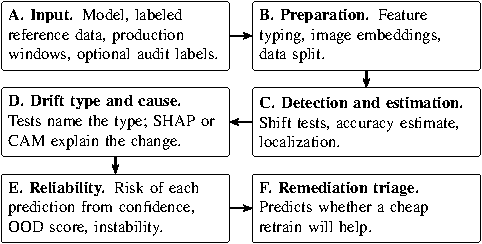
\includegraphics[width=81.6mm,height=0.6\textheight,keepaspectratio]{Fig01.pdf}
\caption{Stages of the monitoring pipeline, from the inputs (A) to the advice on retraining (F)}\label{fig:architecture}
\end{figure}

Stages A to C bring the data into a common form, test whether anything has changed and estimate how much accuracy the change may cost. Stage D, the core of the paper, names the type of change and points to its likely cause. Stages E and F then act on what was found, first for single predictions and then for the decision to retrain. Only the optional audit in stage D uses production labels. With one exception, every decision in the pipeline is a hypothesis test at the significance level $\alpha=0.05$. The exception is the population stability index (PSI), which raises an alarm at a conventional threshold. When many tests are run together, the chance of at least one false alarm is held at $\alpha$ by the Holm procedure~\citep{holm1979}, its weighted form or its Bonferroni bound.

\subsubsection{Notation and drift types}\label{sec:types}

To test for a drift type we first have to say exactly what that type changes. A little notation makes this easier. Write $P(X,Y)$ for the distribution of inputs $X$ and labels $Y$ behind the reference data. A production window (a batch of rows from a later period or from another region) is drawn from $Q(X,Y)$. On every row the model outputs a predicted label $\hat y$ together with a confidence $c$, taken as its largest class probability. The four types differ in what changes between $P$ and $Q$. Covariate shift has $Q(X)\neq P(X)$ while $Q(Y\mid X)=P(Y\mid X)$. Prior shift has $Q(Y)\neq P(Y)$ while $Q(X\mid Y)=P(X\mid Y)$. Concept drift has $Q(Y\mid X)\neq P(Y\mid X)$. Label noise is different again: the true distribution does not move at all, yet each label we observe may have been flipped with some probability. Two more terms recur below. An audit means a random sample of $m$ production rows whose labels come in late. A control window is drawn from the reference distribution itself, so no alarm should fire on it. In practice a real window may carry several types at once; Section~\ref{sec:discussion} comes back to this.

\subsubsection{Reference split, detection and estimation}\label{sec:detection}

Stage C answers three questions: have the data moved, how much accuracy might the change cost and where in the inputs is it located? All three need a clean reference to compare against. The labeled reference data are therefore split into three disjoint parts, stratified by class: 60\% for training, 20\% for calibration and 20\% for testing. The model is fitted on the training part alone. The calibration part is the reference window for every detector and fits the accuracy estimator. The test part gives the reference accuracy and doubles as the control window. Nominal features, such as an occupation code, are treated as categories because their numeric order means nothing. Images are mapped to the 512-dimensional output of the global average pooling layer of a frozen residual network with 18 layers (ResNet-18) trained on ImageNet~\citep{he2016deep}. Image drift can then be tested with the same tests as tabular drift~\citep{rabanser2019failing}.

Six detectors decide whether the inputs or the model outputs have moved. The Kolmogorov--Smirnov (KS) test compares each numeric feature, with a Bonferroni correction over features. PSI raises an alarm at its conventional value of 0.2~\citep{siddiqi2006}. The maximum mean discrepancy (MMD) test~\citep{gretton2012kernel} compares all standardized inputs jointly through a Gaussian kernel, with a permutation p value. The confidence test compares histograms of $c$ with a $\chi^2$ test of homogeneity and pools sparse cells until every expected count reaches 5~\citep{cochran1954}. Two further detectors from Rabanser et al.~\citeyearpar{rabanser2019failing} act as baselines. BBSD applies a KS test to each class probability. The domain classifier trains gradient boosted trees to tell 3,000 reference rows from as many production rows. An exact binomial test then compares its held-out accuracy with $1/2$~\citep{lopezpaz2017c2st}. Every permutation p value is given by $(1+b)/(1+B)$, where $b$ of the $B$ permutations reach the observed statistic~\citep{phipson2010}.

Labels arrive late, so the accuracy is first estimated from the model's own confidence with CBPE~\citep{kivimaki2025performance}. A map $a(\cdot)$ from confidence to the probability of a correct prediction is fitted by histogram binning on the calibration part. For a window with confidences $c_1$ to $c_n$, the estimate $\hat A$ is given by

\begin{equation}
\hat A = \frac{1}{n}\sum_{i=1}^{n} a(c_i).\label{eq:cbpe}
\end{equation}

\noindent A confidence bin that holds fewer than 5 calibration rows cannot give a reliable accuracy, so predictions in such a bin keep their own confidence in Eq.~(\ref{eq:cbpe}). As baselines, AC, DoC and ATC (with the negative entropy score) are fitted on the same calibration part~\citep{hendrycks2017baseline,guillory2021predicting,garg2022atc}.

An alarm helps more when it also says where the change sits. Localization tests every feature, with KS for numeric features and the $\chi^2$ homogeneity test for nominal ones, under Holm correction. It reports an effect size between 0 and 1 for each feature: the KS statistic or Cramér's $V$. For nominal features it also gives the share of production rows whose category never occurs in the reference.

\subsubsection{Drift type diagnosis}\label{sec:diagnosis}

Stage D turns an alarm into one of the four types and thereby into a response. It follows the decision path in Fig.~\ref{fig:decision}. The questions in the upper row use no labels and separate covariate shift from prior shift. The lower row separates concept drift from label noise. It runs only when no label-free test rejects and an audit is available.

\begin{figure}[!htbp]\centering
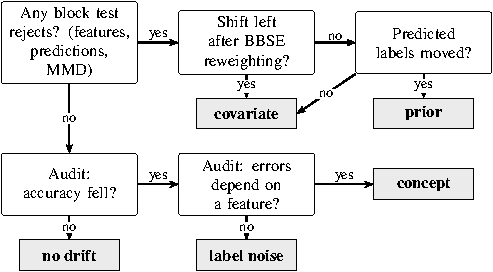
\includegraphics[width=83.5mm,height=0.6\textheight,keepaspectratio]{Fig02.pdf}
\caption{Decision path that names the drift type. Questions are shown in white boxes and verdicts in gray boxes; the upper row needs no labels and the lower row uses the audit}\label{fig:decision}
\end{figure}

\emph{Label-free stage.} The first question is whether anything has moved at all. Three blocks of tests answer it: the feature tests, a $\chi^2$ test on the predicted labels and the MMD test. They form one family tested at level $\alpha$ with a weighted Holm procedure~\citep{holm1979}. The weight starts out split evenly, one third per block. Inside the feature block it is divided again among the individual features. A test that rejects hands its weight on to those still waiting, which is how the family-wise error rate survives every label-free decision. In its first step the procedure reduces to ordinary Holm over the three blocks, each feature block entering through its Bonferroni p value. We pool in this way on purpose. A permutation test cannot return a p value below $1/(B+1)$, so without pooling the MMD test would have little chance against dozens of feature tests. If nothing rejects, the stage stops and reports no shift.

A rejection raises the next question: could a change in the class balance alone produce what we see? To find out, BBSE first estimates the new class prior. Let $C_{jk}=P(\hat y=j,y=k)$ on the calibration part and let $\mu_j$ be the share of production predictions that fall in class $j$. The class weights $w_k=Q(Y=k)/P(Y=k)$ are given by the solution of

\begin{equation}
C\,w = \mu.\label{eq:bbse}
\end{equation}

\noindent If the shift really is a pure prior shift, each class keeps its own input distribution. Reweighting every reference row by the weight $w_{y}$ of its class, as given by Eq.~(\ref{eq:bbse}), ought then to reproduce the production inputs. Checking this is the label shift consistency test, which borrows the prevalence adjustment idea of Roschewitz et al.~\citeyearpar{roschewitz2025shiftid}. The feature tests are repeated against the weighted reference, using Kish's effective sample size~\citep{kish1965} and Holm correction. A feature that still differs carries a covariate shift. If no feature differs and the predicted labels have moved, the shift is a prior shift. A prior shift always moves the predicted labels of an informative classifier, so a shift that leaves them in place is called covariate.

\emph{Audit stage.} Concept drift and label noise do not touch the inputs or the model outputs, so only labels can reveal them. The audit draws $m$ late labels and first checks, with a one-sided two-proportion test, whether accuracy has dropped. If it has, the next question is whether the change in errors depends on a feature. To answer it, a logistic model of whether a prediction is correct is fitted on the calibration rows and the audit rows together. Its null form holds 5 confidence bins at reference quantiles, bins of a feature $f$, an audit indicator and the interaction of that indicator with the confidence bins. The alternative adds the interaction of the indicator with the bins of $f$. A likelihood ratio test compares the two for each feature. A nominal category gets its own bin only if it occurs at least $n_{\min}$ times in the audit, where $n_{\min}$ is given by $\lceil 5/\min(e,1-e)\rceil$ and $e$ is the audit error rate. The remaining categories share one bin.

The confidence term is what separates the two types. In a binary task, uniform label noise at rate $r$ makes the probability of a correct prediction equal to $r+(1-2r)\,q(x)$, where $q(x)$ is the model's own probability of being right at $x$. The change therefore depends on $x$ only through $q(x)$, which the confidence bins of the null absorb. Concept drift, by contrast, moves the errors inside a region of some feature. A feature that stays significant after Holm correction therefore points to concept drift. If no feature is significant, the verdict is label noise. Each of the two stages is tested at level $\alpha$, so a window without drift receives a drift verdict with probability at most $2\alpha$.

\subsubsection{Root cause analysis}\label{sec:rca}

The drift type suggests what kind of fix to consider, but not where the trouble started. Root cause analysis fills that gap by asking which inputs the model now leans on more, or less, than before. The answer narrows the search for a cause without proving one. For tabular models we compute SHAP values~\citep{lundberg2017unified} of the deployed model with its preprocessing and compare the mean absolute attribution of every feature on reference and production rows, each change with a percentile bootstrap interval Bonferroni adjusted over the features. For image models, CAM~\citep{zhou2016cam} highlights the image regions behind the prediction of the linear head.

\subsubsection{Reliability and remediation triage}\label{sec:triage}

Everything so far speaks about a window as a whole. A monitoring team usually wants two more things from it: to know which individual predictions to doubt and whether a cheap retrain would win the accuracy back. For single predictions we combine three signals, each scaled to lie between 0 and 1: the confidence risk $1-c$, the instability of the prediction under small perturbations of the input and an OOD score that blends an Isolation Forest~\citep{liu2008isolation} with a standardized distance. A logistic regression on the calibration part maps the three signals to a probability of error. We fit it only if the calibration part contains at least ten wrong predictions per signal~\citep{peduzzi1996}. With fewer, the risk falls back to $1-c$.

The triage, for its part, has to judge without production labels whether retraining is worth the trouble. It does so with two probes. The first relies on density ratio weights, which come from a classifier trained to tell reference rows from production rows; the weights are fitted on separate folds and capped at 20 times their mean~\citep{cortes2010weights}. A model retrained with them is set against an unweighted model on a held-out 30\% of the reference, weighted in the same way~\citep{shimodaira2000,sugiyama2007}. The second probe needs late labels from an earlier window. Where they exist, it retrains on them and checks the result on a held-out part of that same window. A retrain is recommended only if some probe predicts a gain that stays significant after Holm correction across the probes.

\subsection{Experimental setup}\label{sec:setup}

The experiments are built around two questions. First, does the procedure name the type correctly when the truth is known, including for drift it was not designed for? Second, does it behave sensibly on real drift, where the type is unknown but the causes are on record?

\emph{Protocol.} Every setting below was fixed before the evaluation that uses it. The diagnosis was frozen before the held-out design B was run for the first time. A later review of the code found two errors in the diagnosis. The label-free stage had used a gatekeeping rule whose family-wise error rate reached 6.6\% at a nominal 5\% in a simulation, against 4.9\% for the weighted Holm procedure of Section~\ref{sec:diagnosis}. The audit had also counted nominal categories over the reference rows and audit rows together. Both errors were fixed without looking at the results and every result was produced again, which changed the verdict in 115 of the 5,300 benchmark windows. Permutation tests use 200 permutations. SHAP explains 1,000 rows per side against 100 background rows. Each real audit uses 600 labels from its own random stream. All randomness is seeded, so every result can be repeated exactly. Everything ran on one workstation with a 20-core processor and a graphics processor, using scikit-learn~\citep{pedregosa2011scikit}, SciPy, NumPy, SHAP, OpenCLIP and PyTorch.

\subsubsection{Models}

A diagnosis that worked for only one kind of model would be of limited use, so the pipeline monitors two untuned model families. The first is logistic regression (LR) with $L_2$ regularization ($C=1$) on standardized numeric and one-hot encoded nominal features. The second is histogram gradient boosting (GB)~\citep{ke2017lightgbm} from scikit-learn~\citep{pedregosa2011scikit} with default settings, no early stopping and native splits on nominal codes. Codes beyond the 254 most frequent are pooled, which is the limit of the implementation. For CLEAR-10 both models work on the frozen embeddings. SHAP is reported for LR only, since for GB the exact explainer would take hours per window.

\subsubsection{Datasets}\label{sec:datasets}

The real datasets were chosen because the cause of their drift is documented, which lets us check the verdicts against known events. Table~\ref{tab:datasets} lists the four of them. Two are census tasks from the American Community Survey (ACS) with data from California (CA), Texas (TX), New York (NY), Florida (FL) and Washington (WA). The other two are a gas sensor array and an image stream.

\begin{table}[!htbp]\centering\tablebodyfont
\caption{Datasets, drift windows and reference accuracy}\label{tab:datasets}%
\setlength{\tabcolsep}{4pt}
\begin{tabularx}{\textwidth}{@{}ll>{\raggedright\arraybackslash}Xrrrrr@{}}
\toprule
 &  &  & \multicolumn{1}{c}{} & \multicolumn{1}{c}{} & \multicolumn{1}{c}{} & \multicolumn{2}{c}{Ref. accuracy} \\
\cmidrule(lr){7-8}
Dataset & Reference & Windows & \multicolumn{1}{c}{Rows} & \multicolumn{1}{c}{Inputs} & \multicolumn{1}{c}{Classes} & \multicolumn{1}{c}{LR} & \multicolumn{1}{c}{GB} \\
\midrule
ACS Income & CA 2014 & CA 2015--19 and 2021--23; TX, NY, FL, WA 2014 & 36\,162--203\,278 & 10 & 2 & 0.826 & 0.833 \\
ACS Employment & CA 2014 & CA 2015--19 and 2021--23; TX, NY, FL, WA 2014 & 56\,576--326\,241 & 16 & 2 & 0.729 & 0.772 \\
Gas sensor & batches 1--2 & batches 3--10 & 161--3\,613 & 128 & 6 & 0.982 & 0.985 \\
CLEAR-10 & bucket 1 & buckets 2--10 & 3\,297--3\,300 & 512 & 11 & 0.914 & 0.897 \\
\botrule
\end{tabularx}
\end{table}

Rows gives the smallest and the largest window, Inputs the number of features or embedding dimensions and the last two columns the reference test accuracy of LR and GB.

\emph{ACS Income and ACS Employment.} Both tasks come from the ACS of the United States Census Bureau, as packaged by Folktables~\citep{ding2021retiring}. ACS Income predicts from 10 features whether a person earns more than \$50,000. ACS Employment predicts from 16 features whether a person aged 16 to 90 is employed. CA 2014 is the reference. The temporal windows are CA 2015 to 2019 and 2021 to 2023, as no standard 2020 release exists~\citep{census2021experimental}. The geographic windows are TX, NY, FL and WA in 2014. In 2019 the relationship variable RELP was replaced by RELSHIPP~\citep{census2019pums}. We map it back to RELP with the code labels of the 2018 and 2019 data dictionaries (Table~S2 in Additional file 1). Five documented changes fall in these years: new occupation codes in 2018~\citep{census2020occupation}, a redesigned relationship question in 2019, a new coding of race answers from 2020~\citep{census2021race}, the pandemic and wage growth against the fixed income threshold.

\emph{Gas sensor array drift.} This dataset from the machine learning repository of the University of California, Irvine (UCI) holds 13,910 measurements of six gases by 16 metal oxide sensors, taken over 36 months in ten batches~\citep{vergara2012gas,rodriguezlujan2014gas}. Each measurement has eight features per sensor. As the sensors age, their response to the same gas drifts while the labels stay exact. This is a documented change in $P(X\mid Y)$. Batches 1 and 2 form the reference and batches 3 to 10 the windows. Some batches are small, so the number of audit labels for a window of $n$ rows is given by $\min(600,\lfloor n/2\rfloor)$.

\emph{CLEAR-10.} This image stream has ten object classes and a background class, spread over ten time-ordered buckets of about 3,300 images each~\citep{lin2021clear}. Bucket 1 is the reference.

\subsubsection{Injection benchmark}\label{sec:benchmark-setup}

The type of a real drift is never known for certain, so the diagnosis is graded on drift that we inject ourselves. The benchmark uses the 2014 data of 5 states (CA, TX, NY, FL, WA) for both ACS tasks. Each state acts as a reference distribution with its own model, split as described above. For each of 10 seeds the split, the window and the injection are drawn again, which gives 50 replicates per configuration. A replicate draws a production window of 4,000 rows and a grading holdout of 2,000 rows from the test part. Each mechanism is injected into both at three intensities. The audit uses 600 labels. Proportions carry Wilson intervals~\citep{wilson1927} and means carry bootstrap intervals over replicates.

\emph{Design A} injects the four types in ways that partly match how the tests work. Covariate shift rescales two numeric features (ACS Income: AGEP and WKHP) for a random subset of rows. Prior shift drops rows of one class until the positive rate rises by 0.14, 0.23 and 0.32. Concept drift inverts the labels of the 15, 30 and 50\% of rows with the highest value of one feature (ACS Income: SCHL). Label noise flips a random 8, 18 and 32\% of the labels. Each replicate also contains a control window without drift.

\emph{Design B} uses mechanisms that the tests were not built for. Covariate shift becomes selection bias. Each row is kept with a probability given by $\sigma(\beta s(x))$, where $\sigma$ is the logistic function, $s$ is a seeded random score over all inputs and $\beta\in\{0.5, 1, 1.5\}$. The rows stay real and $P(Y\mid X)$ is exactly unchanged. Prior shift lowers the positive rate by 0.08, 0.14 and 0.20. Concept drift inverts the labels in the top 15, 30 and 50\% of a second random score, which marks out an oblique region that no single feature describes. For ACS Income a second concept drift raises the income threshold to \$55,000, \$60,000 and \$70,000. Label noise is class-conditional: positive labels are flipped to negative at rates of 10, 20 and 35\%.

\subsubsection{Baselines and ablations}\label{sec:baselines}

A diagnosis is only worth running if it does better than simpler options. Every method below names one of the five outcomes (no drift or one of the four types) from the same tests and the same audit labels. Three rules stand for current practice. \emph{Input monitoring} reads any input alarm as covariate shift, which is how drift alarms are commonly read. \emph{BBSE first} reads a shift in the predicted labels as prior shift~\citep{lipton2018bbse,rabanser2019failing} and any other alarm as covariate shift. It is our label-free stage without the consistency test. \emph{Error-rate monitoring} also reads a significant drop in audit accuracy as concept drift, as an error-rate detector would~\citep{gama2004ddm}.

The \emph{learned meta-classifier} checks whether a learned rule could replace the tests. It is a GB model trained on nine statistics of each window: the evidence $-\log_{10}p$ of each block test, the share of features with residual shift, the BBSE prior change, the CBPE change, the evidence and size of the drop in audit accuracy and the evidence of the error structure test. In design A it is validated by leaving one state out. In design B it is trained on design A without the state being predicted, so it never sees a held-out mechanism. Three ablations take parts out of our procedure: the MMD block, the confidence term of the audit null and, in a third variant, the confidence bins, which are replaced by cells of predicted class and confidence.

Each method is compared with ours through the per-replicate difference in the share of correctly typed windows, tested by sign-flip permutation (10,000 flips) with Holm correction. Replicates are the unit of analysis because the windows of one replicate share a model and a reference.

\section{Results}\label{sec:results}

The benchmark comes first: how often the type is named, whether the procedure carries over to drift it was not designed for and how well its building blocks work. Real drift follows.

\subsection{Drift type against baselines}\label{sec:res-methods}

The most direct test of the diagnosis is how often it names the injected type, compared with the baselines. Table~\ref{tab:methods} gives this share for every configuration, each with 50 replicates.

\begin{table}[!htbp]\centering\tablebodyfont
\caption{Share of benchmark windows with the correct drift type (\%)}\label{tab:methods}%
\begin{tabular}{@{}lrrrr@{}}
\toprule
 & \multicolumn{1}{c}{Inc. A} & \multicolumn{1}{c}{Inc. B} & \multicolumn{1}{c}{Emp. A} & \multicolumn{1}{c}{Emp. B} \\
\midrule
\multicolumn{5}{c}{Logistic regression} \\
\midrule
Ours & 94.3 & 62.4 & 85.7 & 80.5 \\
Input monitoring & 30.3$\downarrow$ & 20.0$\downarrow$ & 30.5$\downarrow$ & 25.0$\downarrow$ \\
BBSE first & 30.5$\downarrow$ & 27.7$\downarrow$ & 30.5$\downarrow$ & 39.2$\downarrow$ \\
Error-rate monitoring & 52.3$\downarrow$ & 48.5$\downarrow$ & 52.2$\downarrow$ & 62.8$\downarrow$ \\
Meta-classifier & 97.5 & 31.1$\downarrow$ & 95.8$\uparrow$ & 48.2$\downarrow$ \\
\midrule
Ours, no MMD & 95.2 & 62.9 & 86.6 & 81.3 \\
Ours, no confidence & 79.1$\downarrow$ & 62.9 & 83.7$\downarrow$ & 80.7 \\
Ours, class cells & 93.1 & 65.6$\uparrow$ & 86.2 & 91.8$\uparrow$ \\
\midrule
\multicolumn{5}{c}{Gradient boosting} \\
\midrule
Ours & 94.2 & 63.2 & 90.5 & 81.5 \\
Input monitoring & 30.3$\downarrow$ & 20.0$\downarrow$ & 30.5$\downarrow$ & 25.0$\downarrow$ \\
BBSE first & 30.5$\downarrow$ & 28.1$\downarrow$ & 30.6$\downarrow$ & 40.3$\downarrow$ \\
Error-rate monitoring & 52.5$\downarrow$ & 49.6$\downarrow$ & 53.1$\downarrow$ & 64.8$\downarrow$ \\
Meta-classifier & 98.5$\uparrow$ & 39.2$\downarrow$ & 97.4$\uparrow$ & 51.2$\downarrow$ \\
\midrule
Ours, no MMD & 95.1 & 63.9 & 90.5 & 81.3 \\
Ours, no confidence & 78.0$\downarrow$ & 62.9 & 85.4$\downarrow$ & 82.0 \\
Ours, class cells & 92.9$\downarrow$ & 66.5$\uparrow$ & 90.6 & 93.7$\uparrow$ \\
\botrule
\end{tabular}
\footnotetext{Values are given for each model family, task and design}
\end{table}

Inc. and Emp. stand for ACS Income and ACS Employment. A and B are the two designs. An arrow marks a method that differs significantly from ours after Holm correction: a down arrow means that ours is better and an up arrow that ours is worse. Within each model family the upper block lists the competing methods and the lower block the ablations of our procedure.

With LR on ACS Income, our procedure names the type in 94.3\% of design A windows (95\% interval [92.3, 95.8]). The best rule baseline reaches 52.3\%. The rules are held back by design, since each can name only some of the five outcomes. Over all eight configurations our procedure is significantly better in 28 of the 32 comparisons with a baseline or the learned rule. It is significantly worse in 3, all against the learned meta-classifier on design A (ACS Employment LR, ACS Income GB and ACS Employment GB).

On design A the learned meta-classifier is the strongest competitor. Validated on states it has not seen, it reaches 97.5\% on ACS Income, above our 94.3\%. The held-out mechanisms of design B turn this around. Trained on design A, the meta-classifier drops to 31.1\% on ACS Income and 48.2\% on ACS Employment, while our procedure keeps 62.4\% and 80.5\%. The learned rule had tied each type to the size and shape of the injected shift. It had learned, for example, that covariate shift means a large shift in two features. It therefore misses selection bias, which moves many features a little. This is the main argument for tests over a learned rule. The tests encode what the drift types are, not what the training examples happened to look like.

The overall rates do not show which types get confused with which. Fig.~\ref{fig:confusion} breaks the results down by type for LR.

\begin{figure}[!htbp]\centering
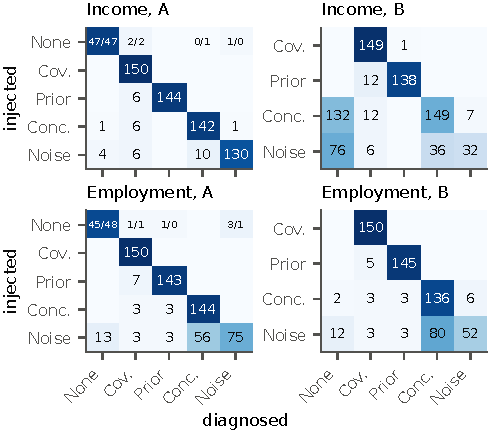
\includegraphics[width=83.5mm,height=0.6\textheight,keepaspectratio]{Fig03.pdf}
\caption{Injected (rows) and diagnosed (columns) drift types on the benchmark with LR. Cells give counts of windows; darker cells hold a larger share of their row}\label{fig:confusion}
\end{figure}

A perfect diagnosis would fill only the diagonal. Design B has no control windows, so false alarms are measured on design A. There, most errors sit in the label noise row, where noise is read either as concept drift or as no drift. The control row holds the false alarms. Our procedure raised one on 13 of 200 control windows (6.5\%), 7 in the label-free stage and 6 in the audit. That is below the bound of 10\% derived in Section~\ref{sec:diagnosis}. In design B the errors gather in the concept and noise rows, for reasons given in Section~\ref{sec:res-mechanisms}.

The ablations show which parts of the procedure carry the weight. Without the confidence term in the audit null, accuracy on ACS Income design A falls by 15.2 points, because uniform label noise then looks like concept drift. Dropping the MMD block changes little on the benchmark (\textminus{}0.9 points), whose shifts are visible feature by feature. Its value shows on the image embeddings of Section~\ref{sec:res-real}. Replacing the confidence bins by cells of predicted class and confidence helps on ACS Employment design B (91.8\% against 80.5\%) but costs accuracy on ACS Income design A (93.1\%). Switching to it now would mean choosing the method after seeing design B. It therefore stays an ablation and a direction for future work.

\subsection{Held-out mechanisms}\label{sec:res-mechanisms}

Design B asks whether the procedure carries over to drift it was not built for. It is the harder of the two tests, since none of its mechanisms shaped any part of the procedure. Table~\ref{tab:mechanisms} gives the results for each mechanism.

\begin{table}[!htbp]\centering\tablebodyfont
\caption{Design B results by drift mechanism}\label{tab:mechanisms}%
\begin{tabular}{@{}lrrrrrrrr@{}}
\toprule
 & \multicolumn{4}{c}{ACS Income} & \multicolumn{4}{c}{ACS Employment} \\
\cmidrule(lr){2-5}
\cmidrule(lr){6-9}
 & \multicolumn{2}{c}{LR} & \multicolumn{2}{c}{GB} & \multicolumn{2}{c}{LR} & \multicolumn{2}{c}{GB} \\
\cmidrule(lr){2-3}
\cmidrule(lr){4-5}
\cmidrule(lr){6-7}
\cmidrule(lr){8-9}
Mechanism & \multicolumn{1}{c}{Corr.} & \multicolumn{1}{c}{Drop} & \multicolumn{1}{c}{Corr.} & \multicolumn{1}{c}{Drop} & \multicolumn{1}{c}{Corr.} & \multicolumn{1}{c}{Drop} & \multicolumn{1}{c}{Corr.} & \multicolumn{1}{c}{Drop} \\
\midrule
Covariate: selection bias & 99 & 0.2 & 99 & 0.3 & 100 & \textminus{}0.3 & 100 & \textminus{}0.3 \\
Prior: decrease & 92 & \textminus{}2.8 & 93 & \textminus{}2.4 & 97 & 2.5 & 97 & 1.9 \\
Concept: oblique region & 95 & 21.9 & 95 & 22.5 & 91 & 15.7 & 97 & 17.7 \\
Concept: income threshold & 4 & \textminus{}0.3 & 6 & 0.2 & -- & -- & -- & -- \\
Noise: class-conditional & 21 & 2.8 & 23 & 3.1 & 35 & 7.7 & 33 & 8.0 \\
\botrule
\end{tabular}
\end{table}

Corr. is the share of windows typed correctly (\%) and Drop is the mean true accuracy drop in points; a negative value means that accuracy rose. The income threshold mechanism exists only for ACS Income.

Three of the five mechanisms carry over well. Selection bias is named covariate shift in 99\% of ACS Income windows with LR, even though no value is distorted and the shift is spread across all features. A lower positive rate is named prior shift in 92\%. Concept drift in an oblique region, which no single feature bounds, is still recognized in 95\%.

The other two mechanisms are harder. A higher threshold relabels some rows in each window, yet model accuracy hardly moves (mean drop \textminus{}0.3 points). With almost nothing lost, the audit stops at its first question and reports no drift in 132 of the 150 windows. This is intended, as the procedure looks for drift that costs accuracy and this drift costs almost none. Class-conditional label noise is recognized in only 21\% of ACS Income windows, for two reasons. At low flip rates the loss of accuracy is too small to show up in 600 labels. At high rates the errors follow the true class, which is itself correlated with the features, so the error structure test reads the pattern as concept drift. A null model built on confidence alone cannot separate the two, a true limitation. Neither failure involves the label-free stage.

Results on ACS Employment and with GB point the same way. On design A the procedure reaches 85.7\% on ACS Employment with LR, while GB brings it to 94.2\% on ACS Income and 90.5\% on ACS Employment. Label noise stays the hardest type there (50.0\% of windows). The ranking of the methods survives the switch of model family, as expected for tests that see only the outputs of the model and its errors.

\subsection{Detection and accuracy estimation}\label{sec:res-detection}

The diagnosis rests on the detectors and on the accuracy estimate, so we also check both on the benchmark. Table~\ref{tab:detectors} gives the alarm rate of each detector for each injected type, pooled over the four design A configurations.

\begin{table}[!htbp]\centering\tablebodyfont
\caption{Detector alarm rates on design A by injected type}\label{tab:detectors}%
\begin{tabular}{@{}lrrrrr@{}}
\toprule
 & \multicolumn{5}{c}{Alarm rate (\%) by injected type} \\
\cmidrule(lr){2-6}
Detector & \multicolumn{1}{c}{No drift [95\% CI]} & \multicolumn{1}{c}{Covariate} & \multicolumn{1}{c}{Prior} & \multicolumn{1}{c}{Concept} & \multicolumn{1}{c}{Noise} \\
\midrule
KS & 1.0 [0.3, 3.6] & 100.0 & 100.0 & 1.0 & 1.0 \\
PSI & 0.0 [0.0, 1.9] & 99.7 & 0.3 & 0.0 & 0.0 \\
MMD & 7.0 [4.2, 11.4] & 100.0 & 100.0 & 7.0 & 7.0 \\
Confidence & 5.0 [2.7, 9.0] & 93.8 & 86.7 & 5.0 & 5.0 \\
BBSD & 2.5 [1.1, 5.7] & 100.0 & 100.0 & 2.5 & 2.5 \\
Domain classifier & 6.0 [3.5, 10.2] & 100.0 & 72.0 & 6.0 & 6.0 \\
\botrule
\end{tabular}
\end{table}

The no drift column is the false alarm rate with its 95\% confidence interval (CI). Over 200 control windows every interval contains $\alpha=0.05$ or lies below it. All detectors catch covariate shift and all except PSI also catch most prior shifts. In concept drift and label noise windows the inputs are the same as in the control window of their replicate, so no detector can see them. This is why the audit is needed. Table~\ref{tab:estimators} turns to the four accuracy estimates and compares them by their mean absolute error against the measured accuracy.

\begin{table}[!htbp]\centering\tablebodyfont
\caption{Mean absolute error of the label-free accuracy estimates (points)}\label{tab:estimators}%
\begin{tabular}{@{}lrrrrrrrr@{}}
\toprule
 & \multicolumn{4}{c}{Benchmark (design A)} & \multicolumn{4}{c}{Real windows} \\
\cmidrule(lr){2-5}
\cmidrule(lr){6-9}
Estimator & \multicolumn{1}{c}{None} & \multicolumn{1}{c}{Cov.} & \multicolumn{1}{c}{Prior} & \multicolumn{1}{c}{Conc., noise} & \multicolumn{1}{c}{Inc.} & \multicolumn{1}{c}{Emp.} & \multicolumn{1}{c}{Gas} & \multicolumn{1}{c}{CLEAR} \\
\midrule
CBPE & \textbf{0.50} & \textbf{9.20} & 3.15 & 14.71 & 1.86 & 1.06 & 30.98 & 0.82 \\
AC & 0.83 & 9.58 & 3.65 & \textbf{14.66} & 1.87 & 1.25 & 30.36 & 5.32 \\
DoC & \textbf{0.50} & 9.63 & 3.12 & 14.71 & 1.77 & 1.06 & 29.78 & 0.76 \\
ATC & 0.63 & 10.31 & \textbf{2.43} & \textbf{14.66} & \textbf{1.15} & \textbf{1.02} & \textbf{26.95} & \textbf{0.62} \\
\botrule
\end{tabular}
\end{table}

Cov. and Conc. stand for covariate shift and concept drift, Inc. and Emp. for the two ACS tasks. The smallest error in each column is in bold. On design A all four estimates stay within 0.83 points without drift and within 10.31 points under covariate shift. Under concept drift and label noise every error equals the whole loss, about 14.71 points, because the inputs do not change. Across these 8 comparisons ATC has the smallest error in 6 and CBPE in only 2. On the gas sensor data all four miss by 26.95 to 30.98 points on average. In batch 8 the mean confidence of the LR model falls from 0.973 to 0.595 and its accuracy to 0.330, yet CBPE estimates 0.618. The estimate is best read as an upper bound on accuracy.

\subsection{Real drift}\label{sec:res-real}

On real data the type of drift is not known, but its causes are on record. Here we ask whether the verdicts agree with those causes and whether the control windows stay quiet. Fig.~\ref{fig:timelines} shows how accuracy changes over time in all four datasets.

\begin{figure}[!htbp]\centering
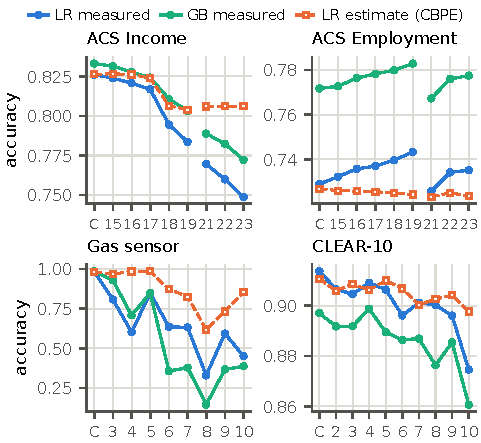
\includegraphics[width=83.5mm,height=0.6\textheight,keepaspectratio]{Fig04.pdf}
\caption{Measured accuracy of both models and the label-free CBPE estimate on the temporal windows}\label{fig:timelines}
\end{figure}

C marks the control window. The numbers mark years (ACS), batches (gas sensor) or buckets (CLEAR-10). The gap in the ACS lines is the missing 2020 release.

ACS Income shows the clearest trend, so we start there. Its accuracy falls over time for both models, with LR going from 0.824 in 2015 to 0.749 in 2023, while the CBPE estimate falls far less. Table~\ref{tab:income} lists the details behind the ACS Income panel of Fig.~\ref{fig:timelines}.

\begin{table}[!htbp]\centering\tablebodyfont
\caption{Detection and diagnosis on the ACS Income windows}\label{tab:income}%
\begin{tabular}{@{}lrrrcccccll@{}}
\toprule
 & \multicolumn{3}{c}{Accuracy} & \multicolumn{5}{c}{Alarms} &  &  \\
\cmidrule(lr){2-4}
\cmidrule(lr){5-9}
Window & \multicolumn{1}{c}{$\Delta$LR} & \multicolumn{1}{c}{$\Delta$GB} & \multicolumn{1}{c}{Est. err.} & \multicolumn{1}{c}{K} & \multicolumn{1}{c}{M} & \multicolumn{1}{c}{C} & \multicolumn{1}{c}{B} & \multicolumn{1}{c}{D} & Top shifts & Type \\
\midrule
Control & 0.0 & 0.0 & 0.0 & -- & -- & -- & -- & -- & -- & -- \\
2015 & \textminus{}0.2 & \textminus{}0.2 & +0.3 & \checkmark{} & -- & -- & -- & -- & OCCP & -- \\
2016 & \textminus{}0.5 & \textminus{}0.5 & +0.6 & \checkmark{} & -- & -- & \checkmark{} & \checkmark{} & OCCP,~POBP & Cov. \\
2017 & \textminus{}0.9 & \textminus{}0.9 & +0.7 & \checkmark{} & \checkmark{} & \checkmark{} & \checkmark{} & -- & OCCP,~POBP & Cov. \\
2018 & \textminus{}3.2 & \textminus{}2.2 & +1.2 & \checkmark{} & \checkmark{} & \checkmark{} & \checkmark{} & \checkmark{} & OCCP,~POBP & Cov. \\
2019 & \textminus{}4.2 & \textminus{}3.0 & +2.0 & \checkmark{} & \checkmark{} & \checkmark{} & \checkmark{} & \checkmark{} & OCCP,~RELP & Cov. \\
2021 & \textminus{}5.6 & \textminus{}4.4 & +3.6 & \checkmark{} & \checkmark{} & \checkmark{} & \checkmark{} & \checkmark{} & OCCP,~RAC1P & Cov. \\
2022 & \textminus{}6.6 & \textminus{}5.1 & +4.6 & \checkmark{} & \checkmark{} & \checkmark{} & \checkmark{} & \checkmark{} & OCCP,~RAC1P & Cov. \\
2023 & \textminus{}7.7 & \textminus{}6.1 & +5.7 & \checkmark{} & \checkmark{} & \checkmark{} & \checkmark{} & \checkmark{} & OCCP,~RAC1P & Cov. \\
TX & \textminus{}2.4 & \textminus{}2.7 & +1.1 & \checkmark{} & \checkmark{} & \checkmark{} & \checkmark{} & \checkmark{} & POBP,~RAC1P & Cov. \\
NY & \textminus{}2.2 & \textminus{}2.7 & +0.8 & \checkmark{} & \checkmark{} & \checkmark{} & \checkmark{} & \checkmark{} & POBP,~RAC1P & Cov. \\
FL & \textminus{}4.0 & \textminus{}4.3 & +2.2 & \checkmark{} & \checkmark{} & \checkmark{} & \checkmark{} & \checkmark{} & POBP,~RAC1P & Cov. \\
WA & \textminus{}2.5 & \textminus{}2.5 & +0.9 & \checkmark{} & \checkmark{} & \checkmark{} & \checkmark{} & \checkmark{} & POBP,~RAC1P & Cov. \\
\botrule
\end{tabular}
\footnotetext{The alarms are those of the LR model: K is the KS test, M the MMD test, C the confidence test, B BBSD and D the domain classifier}
\end{table}

The years are the California windows and TX, NY, FL and WA the 2014 windows of the other states. $\Delta$ is the change in accuracy, in points, against each model's accuracy on the control window. Est. err. is the error of the CBPE estimate. A tick marks an alarm. Type is the verdict of the diagnosis, the same for LR and GB in every window (Cov. is covariate shift). Top shifts lists the two features with the largest effect size: occupation (OCCP), place of birth (POBP), relationship (RELP) and race (RAC1P).

Neither model raises an alarm on the control window. Both call CA 2015, whose accuracy did not change significantly, no drift and every other window covariate shift. The documented events can be read off the localization. The 2018 revision of the occupation codes left 26.6\% of rows with a code that never occurred in 2014. Occupation lost weight in the model as a result (SHAP change \textminus{}0.032). Relationship moves in 2019 (effect size 0.091), when its survey question was redesigned. Race moves from 2021 (effect size 0.186), once the Census Bureau had changed its coding of written race answers~\citep{census2021race}. Wage growth, measured against a fixed income threshold, shows up in the labels instead: their positive share rises from 0.355 in the control window to 0.498 in 2023 while the model predicts only 0.338. Part of the 2023 loss comes from a change in what the labels mean, something no label-free test can detect.

The cost of a drift differs widely between datasets. On ACS Employment every window is diagnosed as covariate shift, yet LR accuracy never changes by more than 2.2 points; relationship (2019) and race (from 2021) shift there as well while the model barely responds. Here an alarm alone would overstate the problem; the accuracy estimate and the audit keep it in proportion. The gas sensor batches all come out as covariate shift too, as they should for aging sensors that alter $P(X\mid Y)$. The largest loss is in batch 8 (\textminus{}65.2 points for LR). BBSE at first takes each gas batch for a prior shift, since the predicted labels move too. The consistency test corrects this: the sensors respond differently to a gas mix that has not changed.

CLEAR-10 drifts more gently: buckets 2 and 3 show no drift for either model, while buckets 4, 5, 6, 7, 8, 9 and 10 show covariate shift. In buckets 4, 5, 6 and 9 no single embedding dimension shifts significantly with LR. Only the MMD test sees the change while the predicted labels stay put, which is why the multivariate block is needed. The only detector alarm on any control window comes from the domain classifier baseline on CLEAR-10 ($p=0.034$), a false alarm of the kind that $\alpha$ allows.

\subsection{Reliability and triage}\label{sec:res-reliability}

The last two stages act on single predictions and on retraining. The fused risk score is judged by how well it ranks wrong predictions above right ones. Where the fusion is learned, on ACS and CLEAR-10, its area under the receiver operating characteristic curve (AUROC) differs from that of confidence alone by \textminus{}0.012 to +0.001 over 72 windows and by \textminus{}0.002 to +0.009 on the benchmark. On the gas sensor array the calibration part holds too few wrong predictions (4 with LR and 11 with GB), so the risk falls back to confidence. Confidence alone carries most of the information about a single prediction.

For the triage, a retrain truly helps when importance weighting or the latest labeled window raises holdout accuracy significantly. Over 82 real settings (Table~S1 in Additional file 1), the triage is right in 54 of the 58 settings that have an earlier labeled window, because its recent-window probe is checked on real labels. Without such a window it relies on importance-weighted validation. It is then right in 23 of 24 settings, but mostly by advising against a retrain, since one truly helped in only 2 of them. On the benchmark its recall is 6\%, because importance-weighted validation cannot see gains outside the reference data. A dashboard presents all of these results step by step (Fig.~S2 in Additional file 1).

\section{Discussion}\label{sec:discussion}

On injected drift the procedure beats rules from monitoring practice and the label shift literature and works for both model families. Unlike a learned meta-classifier, it also carries over to held-out drift, because the tests encode the definitions of the types. On real drift it reported no drift on any control window and traced documented events, from new occupation codes to aging sensors.

Several limits apply. Each benchmark window holds a single type, while real windows such as ACS Income 2023 mix several. The four types are also an idealization: sensor aging changes $P(X\mid Y)$ and, through it, $P(Y\mid X)$, yet our procedure reports it as covariate shift. Design B reduces, but cannot remove, the risk that the benchmark favors the tests. The weighted residual tests do not account for the sampling error of the BBSE weights. At several hundred thousand rows almost any shift is significant, so each decision carries an effect size. The audit lets through drift that does not hurt accuracy and often mistakes class-conditional label noise for concept drift. Deep models trained end to end, text and streaming data remain untested.

\section{Conclusions}\label{sec:conclusions}

This paper showed that hypothesis tests with a stated error rate can name the drift type, which decides the right response, from label-free tests and a few hundred late labels. The next steps are an audit conditioned on the full model output, a model of the sampling error of the BBSE weights and benchmark windows that mix several types.

\section*{Supplementary information}

\textbf{Additional file 1} (PDF). Supplementary material. Size of the delayed audit (Fig.~S1), remediation triage by real setting (Table~S1), the mapping of the ACS relationship codes across the 2019 redesign (Table~S2) and the dashboard of the pipeline (Fig.~S2).

\section*{List of abbreviations}

AC: Average confidence; ACS: American Community Survey; ATC: Average thresholded confidence; AUROC: Area under the receiver operating characteristic curve; BBSD: Black-box shift detection; BBSE: Black-box shift estimation; CA: California; CAM: Class activation maps; CBPE: Confidence-based performance estimation; CI: Confidence interval; CLEAR: Continual LEArning on Real-World Imagery; DDM: Drift detection method; DoC: Difference of confidences; FL: Florida; GB: Histogram gradient boosting; Grad-CAM: Gradient-weighted class activation mapping; KS: Kolmogorov--Smirnov; LR: Logistic regression; MMD: Maximum mean discrepancy; NY: New York; OCCP: Occupation (ACS variable); OOD: Out-of-distribution; POBP: Place of birth (ACS variable); PSI: Population stability index; RAC1P: Race (ACS variable); RELP: Relationship (ACS variable); SHAP: Shapley additive explanations; TX: Texas; UCI: University of California, Irvine; WA: Washington

\section*{Declarations}

\bmhead{Ethics approval and consent to participate}

Not applicable.

\bmhead{Consent for publication}

Not applicable.

\bmhead{Availability of data and materials}

The datasets analyzed in this study are available in public repositories. The American Community Survey microdata are published by the U.S. Census Bureau~\citep{census2026pums} and were obtained with the Folktables package~\citep{ding2021retiring}. The gas sensor array drift dataset is available in the UCI Machine Learning Repository, \url{https://doi.org/10.24432/C5RP6W}~\citep{vergara2012gasdata}. The CLEAR-10 benchmark is available from its project page, \url{https://clear-benchmark.github.io/}~\citep{lin2021clear}. The code that supports the conclusions of this article is available as follows. Project name: Data Drift Autopsy. Project home page: \url{https://github.com/NathanC987/data-drift-autopsy}. Archived version: \textcolor{red}{DOI of the release archived on Zenodo}. Operating system: platform independent. Programming language: Python. Other requirements: Python 3.10 or higher with NumPy, pandas, SciPy and scikit-learn; SHAP, PyTorch, torchvision, OpenCLIP and Streamlit for the explanations, the image models and the dashboard. License: MIT. Restrictions to use by non-academics: none.

\bmhead{Competing interests}

The authors declare that they have no competing interests.

\bmhead{Funding}

This research received no external funding.

\bmhead{Authors' contributions}

RG designed and implemented the reliability layer, which scores the risk of each prediction, implemented the label-free accuracy estimators with their baselines and ran the CLEAR-10 study. NC designed the hierarchical diagnosis with the delayed label audit, built the drift injection benchmark with its baselines and the meta-classifier and ran the gas sensor study. AkP implemented the feature localization tests and the root cause analysis, with SHAP attributions for the tabular models and gradient-weighted class activation maps (Grad-CAM) for the image model. AlP implemented the remediation triage, which compares importance weighting with retraining on recent or audit labels, the monitoring dashboard and the ACS studies, including the mapping of the relationship codes across the 2019 redesign. RG, NC, AkP and AlP drafted and revised the manuscript together. SM supervised the project and critically reviewed the manuscript. All authors read and approved the final manuscript.

\bmhead{Acknowledgements}

Not applicable.

\bibliography{references}

\end{document}
